\documentclass[tikz,border=5pt]{standalone}
\usepackage[T1]{fontenc}
\usepackage{lmodern,amsmath,amssymb}
\usetikzlibrary{arrows.meta,calc,positioning,fit,backgrounds,shapes.geometric,matrix,decorations.pathreplacing,patterns}
\definecolor{ink}{gray}{0.08}
\definecolor{wash}{gray}{0.965}
\definecolor{soft}{gray}{0.45}
\tikzset{box/.style={draw=ink,line width=.65pt,fill=white,align=center,inner sep=4pt,outer sep=0pt,font=\small},flow/.style={draw=ink,line width=.65pt,-{Latex[length=1.8mm,width=1.3mm]},rounded corners=2pt},annotation/.style={font=\scriptsize,text=soft,align=center},groupbox/.style={draw=soft,dashed,line width=.45pt,fill=wash}}
\begin{document}
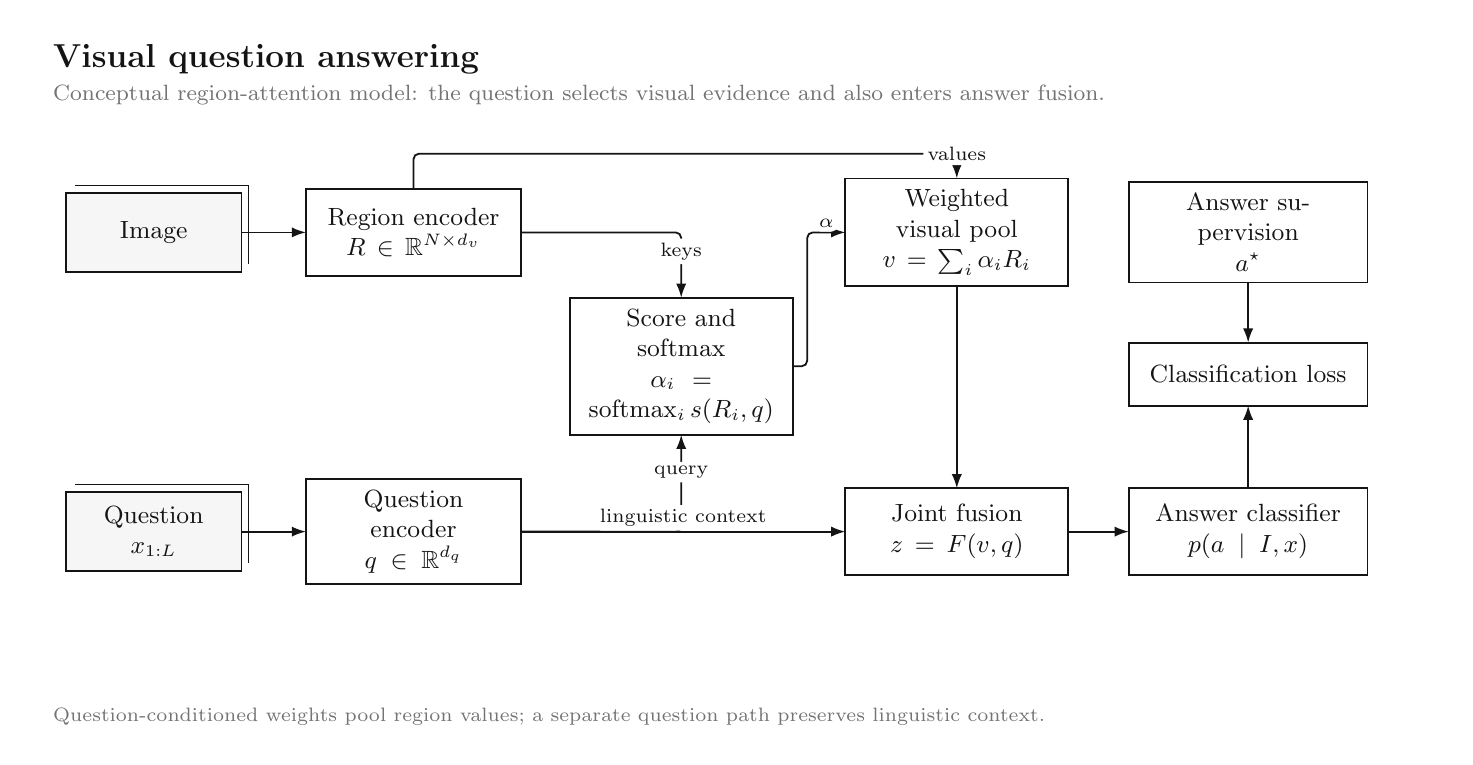
\begin{tikzpicture}[x=1cm,y=-1cm,font=\rmfamily,text=ink]

\path[use as bounding box] (0,0) rectangle (18,9);
\node[anchor=west,font=\large\bfseries] at (.2,.4) {Visual question answering};
\node[anchor=west,font=\footnotesize,text=soft] at (.2,.85) {Conceptual region-attention model: the question selects visual evidence and also enters answer fusion.};
\begin{pgfonlayer}{background}
\end{pgfonlayer}
\node[box,fill=wash,minimum width=2.2cm,minimum height=1cm,text width=1.9500000000000002cm] (image) at (1.6,2.6) {Image};
\draw[ink,line width=.4pt] (0.6,2.0) -- (2.8000000000000003,2.0) -- (2.8000000000000003,3.0);
\node[box,minimum width=2.7cm,minimum height=1.1cm,text width=2.45cm] (regions) at (4.9,2.6) {Region encoder\\$R\in\mathbb{R}^{N\times d_v}$};
\node[box,fill=wash,minimum width=2.2cm,minimum height=1cm,text width=1.9500000000000002cm] (question) at (1.6,6.4) {Question\\$x_{1:L}$};
\draw[ink,line width=.4pt] (0.6,5.800000000000001) -- (2.8000000000000003,5.800000000000001) -- (2.8000000000000003,6.800000000000001);
\node[box,minimum width=2.7cm,minimum height=1.1cm,text width=2.45cm] (qenc) at (4.9,6.4) {Question encoder\\$q\in\mathbb{R}^{d_q}$};
\node[box,minimum width=2.8cm,minimum height=1.3cm,text width=2.55cm] (att) at (8.3,4.3) {Score and softmax\\$\alpha_i=\mathrm{softmax}_i\,s(R_i,q)$};
\node[box,minimum width=2.8cm,minimum height=1.1cm,text width=2.55cm] (pool) at (11.8,2.6) {Weighted visual pool\\$v=\sum_i\alpha_iR_i$};
\node[box,minimum width=2.8cm,minimum height=1.1cm,text width=2.55cm] (fuse) at (11.8,6.4) {Joint fusion\\$z=F(v,q)$};
\node[box,minimum width=3.0cm,minimum height=1.1cm,text width=2.75cm] (answer) at (15.5,6.4) {Answer classifier\\$p(a\mid I,x)$};
\node[box,minimum width=3.0cm,minimum height=1cm,text width=2.75cm] (target) at (15.5,2.6) {Answer supervision\\$a^{\star}$};
\node[box,minimum width=3.0cm,minimum height=0.8cm,text width=2.75cm] (loss) at (15.5,4.4) {Classification loss};
\begin{pgfonlayer}{background}
\draw[flow] (image.east) -- (regions.west);
\draw[flow] (question.east) -- (qenc.west);
\draw[flow] (regions.east) -- (8.3,2.6) -- (att.north) node[midway,above,fill=white,inner sep=1.5pt,font=\scriptsize] {keys};
\draw[flow] (qenc.east) -- (8.3,6.4) -- (att.south) node[midway,above,fill=white,inner sep=1.5pt,font=\scriptsize] {query};
\draw[flow] (regions.north) -- (4.9,1.6) -- (11.8,1.6) -- (pool.north) node[midway,above,fill=white,inner sep=1.5pt,font=\scriptsize] {values};
\draw[flow] (att.east) -- (9.9,4.3) -- (9.9,2.6) -- (pool.west) node[midway,above,fill=white,inner sep=1.5pt,font=\scriptsize] {$\alpha$};
\draw[flow] (pool.south) -- (fuse.north);
\draw[flow] (qenc.east) -- (fuse.west) node[midway,above,fill=white,inner sep=1.5pt,font=\scriptsize] {linguistic context};
\draw[flow] (fuse.east) -- (answer.west);
\draw[flow] (target.south) -- (loss.north);
\draw[flow] (answer.north) -- (loss.south);
\end{pgfonlayer}
\node[anchor=west,align=left,font=\scriptsize,text=soft,text width=17.6cm] at (.2,8.75) {Question-conditioned weights pool region values; a separate question path preserves linguistic context.};
\end{tikzpicture}
\end{document}
